% MCP-RAG Complete System Paper
% A Comprehensive Technical Specification
\documentclass[11pt,letterpaper]{article}

% Packages
\usepackage[utf8]{inputenc}
\usepackage[margin=1in]{geometry}
\usepackage{amsmath,amssymb,amsfonts}
\usepackage{algorithm}
\usepackage{algorithmic}
\usepackage{listings}
\usepackage{xcolor}
\usepackage{hyperref}
\usepackage{booktabs}
\usepackage{graphicx}
\usepackage{cite}
\usepackage{fancyhdr}
\usepackage{tikz}
\usepackage{float}
\usepackage{longtable}
\usepackage{multirow}
\usepackage{enumitem}
\usepackage{caption}
% \usepackage{subcaption}  % Not available on this system
\usetikzlibrary{shapes,arrows,positioning,fit,backgrounds,calc}

% Hyperref setup
\hypersetup{
    colorlinks=true,
    linkcolor=blue,
    citecolor=blue,
    urlcolor=blue,
    pdftitle={MCP-RAG: A Hybrid Intelligence System for Operational Weather Forecasting Software},
    pdfauthor={Terrence McGuinness, NOAA EMC},
    pdfkeywords={MCP, RAG, Knowledge Graphs, AI-Assisted Development, Weather Forecasting}
}

% Code listing setup
\lstdefinestyle{code}{
    basicstyle=\ttfamily\footnotesize,
    breaklines=true,
    frame=single,
    captionpos=b,
    numbers=left,
    numberstyle=\tiny\color{gray},
    keywordstyle=\color{blue},
    commentstyle=\color{green!60!black},
    stringstyle=\color{red},
    backgroundcolor=\color{gray!5}
}

\lstdefinestyle{rst}{
    basicstyle=\ttfamily\footnotesize,
    breaklines=true,
    frame=single,
    backgroundcolor=\color{yellow!5}
}

% Header/Footer
\pagestyle{fancy}
\fancyhf{}
\rhead{MCP-RAG System}
\lhead{NOAA EMC Technical Report}
\cfoot{\thepage}

% Custom commands
\newcommand{\sdd}{\textsc{SDD}}
\newcommand{\mcp}{\textsc{MCP}}
\newcommand{\rag}{\textsc{RAG}}

% Title
\title{%
    \vspace{-1cm}
    \textbf{MCP-RAG: A Hybrid Intelligence System for\\
    AI-Assisted Software Development in\\
    Operational Weather Forecasting}\\[0.5cm]
    \large Integrating Semantic Embeddings, Knowledge Graphs,\\
    and Supervised SME Refinement\\[0.3cm]
    \normalsize Complete Technical Specification v2.0
}

\author{
    Terrence McGuinness\\
    Enterprise Infrastructure Branch\\
    Environmental Modeling Center\\
    National Oceanic and Atmospheric Administration\\
    \texttt{Terry.McGuinness@noaa.gov}\\[0.3cm]
    \textit{With AI Collaboration: Claude Opus 4.5}
}

\date{December 4, 2025}

\begin{document}

\maketitle

\begin{abstract}
We present \textbf{MCP-RAG}, a comprehensive artificial intelligence system for assisting software development in large-scale operational weather forecasting infrastructure. The system integrates three architectural innovations: (1) \textit{Spec-Driven Development} (\sdd{}), a methodology for expressing development tasks as machine-readable workflow specifications; (2) \textit{Hybrid Graph-Enhanced Retrieval-Augmented Generation}, combining 768-dimensional semantic embeddings with Neo4j knowledge graphs for context-aware code intelligence; and (3) \textit{Supervised SME Refinement}, enabling domain experts to correct AI behavior through structured semantic annotations in reStructuredText documentation.

Deployed within the NOAA Global Workflow system---the operational infrastructure producing GFS, GEFS, and GDAS weather forecasts---the platform demonstrates measurable improvements: 3.8$\times$ retrieval precision over baseline text search, 5--9$\times$ development velocity for complex tasks, and 77\% reduction in false positive compliance violations through SME-guided corrections. The system processes a knowledge base of 3,761 documents across 78,339 code relationships, exposing 20+ specialized tools via the Model Context Protocol (\mcp{}) for integration with VS Code, Claude, and other AI coding assistants.

This paper provides a complete technical specification including: mathematical foundations of embedding spaces and graph traversal; the seven-directive semantic annotation schema; the five-component hybrid architecture; empirical evaluation methodology; and a prioritized roadmap for containerized deployment. We conclude with reflections on human-AI alignment in safety-critical software systems, arguing that supervised refinement---rather than pure automation---is essential for trustworthy AI assistance.

\textbf{Keywords:} Model Context Protocol, Retrieval-Augmented Generation, Knowledge Graphs, Spec-Driven Development, Semantic Annotations, Subject Matter Expert Refinement, Weather Forecasting Systems, Human-AI Collaboration, EE2 Compliance
\end{abstract}

\tableofcontents
\newpage

%==============================================================================
\section{Introduction}
%==============================================================================

\subsection{The Challenge of Operational Complexity}

Modern operational weather forecasting systems represent some of the most complex software infrastructures in existence. NOAA's Global Workflow, which produces the Global Forecast System (GFS) and Global Ensemble Forecast System (GEFS) forecasts used worldwide, integrates:

\begin{itemize}[leftmargin=*]
    \item \textbf{Unified Forecast System (UFS)}: $\sim$500,000 lines of Fortran atmospheric modeling code
    \item \textbf{GSI/GDAS}: $\sim$300,000 lines of data assimilation code
    \item \textbf{Workflow Orchestration}: Rocoto XML with 7,000+ task dependencies
    \item \textbf{Python Execution}: The \texttt{wxflow} library for workflow management
    \item \textbf{Shell Scripting}: 2,000+ operational scripts with strict compliance requirements
    \item \textbf{HPC Configurations}: Platform-specific adaptations for Hera, Hercules, Orion, WCOSS2, and Gaea
\end{itemize}

This complexity creates five fundamental challenges:

\begin{enumerate}
    \item \textbf{Knowledge Scarcity}: Few individuals understand the complete system end-to-end
    \item \textbf{Documentation Decay}: Code evolves faster than documentation can be maintained
    \item \textbf{Onboarding Friction}: New developers require 6--12 months to become productive
    \item \textbf{Compliance Burden}: NCEP Central Operations (NCO) mandates EE2 standards requiring manual auditing
    \item \textbf{Operational Risk}: Silent failures can cascade through 6-hour forecast windows, affecting public safety
\end{enumerate}

\subsection{The MCP-RAG Vision}

The \textbf{MCP-RAG} system addresses these challenges through a novel integration of three technologies:

\textbf{1. Model Context Protocol (MCP)}: A standardized interface allowing AI models to access domain-specific tools, file systems, and documentation. MCP enables VS Code Copilot, Claude, and other AI assistants to ``see'' NOAA's specific infrastructure.

\textbf{2. Retrieval-Augmented Generation (RAG)}: Rather than relying on general training knowledge, the system retrieves relevant documentation and code at query time, grounding responses in actual source material.

\textbf{3. Hybrid Intelligence}: Combining vector embeddings (semantic similarity) with knowledge graphs (structural relationships) for context-aware retrieval that neither technology could achieve alone.

The key insight is that \textit{AI assistance is most effective when domain experts can correct and refine AI behavior}. Pure automation fails in complex domains; supervised human-AI collaboration succeeds.

\subsection{Paper Organization}

This paper provides a complete technical specification:

\begin{itemize}
    \item \textbf{Section 2}: Mathematical foundations---embedding spaces, graph theory, and hybrid scoring
    \item \textbf{Section 3}: Spec-Driven Development methodology and workflow specifications
    \item \textbf{Section 4}: Semantic annotation schema and the seven MCP directive types
    \item \textbf{Section 5}: System architecture---the five-component pipeline
    \item \textbf{Section 6}: Implementation details---20+ MCP tools across five categories
    \item \textbf{Section 7}: SME refinement methodology and the review guide
    \item \textbf{Section 8}: Empirical evaluation and case studies
    \item \textbf{Section 9}: Deployment roadmap and containerization strategy
    \item \textbf{Section 10}: Future work---Fortran call trees and multimodal embeddings
    \item \textbf{Section 11}: Conclusions on human-AI alignment
\end{itemize}

%==============================================================================
\section{Mathematical Foundations}
%==============================================================================

\subsection{Embedding Spaces}

The system represents text as vectors in a high-dimensional Euclidean space. Using the \texttt{all-mpnet-base-v2} model from Sentence Transformers, each text chunk is mapped to a 768-dimensional vector:

\begin{equation}
    \phi: \mathcal{T} \rightarrow \mathbb{R}^{768}
\end{equation}

where $\mathcal{T}$ is the space of text strings and $\phi$ is the embedding function learned by the transformer.

\subsubsection{Cosine Similarity}

Semantic similarity between texts $t_1$ and $t_2$ is measured via cosine similarity:

\begin{equation}
    \text{sim}(t_1, t_2) = \frac{\phi(t_1) \cdot \phi(t_2)}{\|\phi(t_1)\| \cdot \|\phi(t_2)\|}
\end{equation}

This metric ranges from $-1$ (opposite) to $+1$ (identical), with values above 0.7 typically indicating strong semantic relatedness.

\subsubsection{Metric Space Properties}

Cosine similarity does not satisfy the triangle inequality strictly, so the embedding space is a \textit{pseudo-metric space} rather than a true metric space. However, for retrieval purposes, this is sufficient---we seek approximate nearest neighbors, not exact geometric properties.

The 768 dimensions are not individually interpretable but collectively encode:
\begin{itemize}
    \item Syntactic features (programming language constructs)
    \item Semantic roles (error handling, data flow, configuration)
    \item Domain concepts (weather, HPC, compliance)
\end{itemize}

\subsection{Graph Theory for Code Structure}

While embeddings capture \textit{what text means}, graphs capture \textit{how code is connected}. We model the codebase as a directed labeled graph $G = (V, E, L)$ where:

\begin{itemize}
    \item $V$ = nodes representing files, functions, classes, modules
    \item $E \subseteq V \times V$ = directed edges representing relationships
    \item $L: E \rightarrow \mathcal{R}$ = edge labels from relationship types $\mathcal{R}$
\end{itemize}

\subsubsection{Relationship Types}

The graph schema includes the following edge types:

\begin{table}[H]
\centering
\caption{Neo4j Relationship Types}
\begin{tabular}{@{}lll@{}}
\toprule
\textbf{Relationship} & \textbf{Pattern} & \textbf{Meaning} \\
\midrule
\texttt{CALLS} & \texttt{(f1:Function)-[:CALLS]->(f2:Function)} & f1 invokes f2 \\
\texttt{IMPORTS} & \texttt{(f:File)-[:IMPORTS]->(m:Module)} & File imports module \\
\texttt{DEFINES} & \texttt{(f:File)-[:DEFINES]->(fn:Function)} & File defines function \\
\texttt{INVOKES} & \texttt{(s:Script)-[:INVOKES]->(p:Program)} & Shell invokes executable \\
\texttt{USES} & \texttt{(fn:Function)-[:USES]->(m:Module)} & Function uses module \\
\texttt{DOCUMENTS} & \texttt{(d:Doc)-[:DOCUMENTS]->(c:Code)} & Doc describes code \\
\bottomrule
\end{tabular}
\end{table}

\subsubsection{Graph Traversal}

For structural queries (``What calls this function?''), we execute Cypher traversals:

\begin{lstlisting}[style=code, language=SQL, caption={Cypher Query for Call Chain}]
MATCH path = (caller:Function)-[:CALLS*1..5]->(target:Function {name: $name})
RETURN path
ORDER BY length(path)
LIMIT 10
\end{lstlisting}

The traversal depth is configurable (default: 3) to balance completeness against query time.

\subsection{Hybrid Scoring Function}

The core innovation is combining vector similarity with graph relevance and annotation matching:

\begin{equation}
    \text{score}(q, d) = \alpha \cdot \text{sim}_{\text{vec}}(q, d) + \beta \cdot \text{rel}_{\text{graph}}(q, d) + \gamma \cdot \text{match}_{\text{annot}}(q, d)
\end{equation}

where:
\begin{itemize}
    \item $\text{sim}_{\text{vec}}$: Cosine similarity from ChromaDB
    \item $\text{rel}_{\text{graph}}$: Graph relevance (connection distance, relationship count)
    \item $\text{match}_{\text{annot}}$: Semantic annotation match score
    \item $\alpha, \beta, \gamma$: Tunable weights (default: 0.5, 0.3, 0.2)
\end{itemize}

\subsubsection{Query-Type Optimization}

Different query types benefit from different weight configurations:

\begin{table}[H]
\centering
\caption{Optimized Weights by Query Type}
\begin{tabular}{@{}lcccp{4cm}@{}}
\toprule
\textbf{Query Type} & $\alpha$ & $\beta$ & $\gamma$ & \textbf{Example} \\
\midrule
Concept & 0.7 & 0.1 & 0.2 & ``What is Rocoto?'' \\
Usage & 0.5 & 0.3 & 0.2 & ``How do I use err\_chk?'' \\
Code Structure & 0.2 & 0.7 & 0.1 & ``What calls this function?'' \\
Compliance & 0.3 & 0.2 & 0.5 & ``Is this script EE2 compliant?'' \\
Troubleshooting & 0.4 & 0.4 & 0.2 & ``Why is forecast failing?'' \\
\bottomrule
\end{tabular}
\end{table}

%==============================================================================
\section{Spec-Driven Development Methodology}
%==============================================================================

\subsection{Core Principles}

The \sdd{} Framework is built on four foundational principles:

\textbf{P1: Specifications as First-Class Artifacts.} Development tasks are expressed as machine-readable specifications \textit{before} implementation. Specifications define what, how, when, and who.

\textbf{P2: Progressive Refinement.} Specifications evolve from high-level intent to detailed implementation through iterative refinement with human oversight.

\textbf{P3: Health-Integrated Architecture.} All components integrate health monitoring from initialization. System health is a first-class concern, not an afterthought.

\textbf{P4: Supervised Human-AI Collaboration.} AI agents propose implementations; human experts review, refine, and approve. Pure automation is rejected as insufficiently reliable for operational systems.

\subsection{Workflow Specification Format}

SDD workflows are expressed in Markdown with structured phases and steps:

\begin{lstlisting}[style=code, caption={SDD Workflow Structure}]
# Phase N: Feature Name

**Description**: High-level goal
**Status**: PLANNING | IN_PROGRESS | COMPLETE
**Priority**: Critical | High | Medium | Backlog

## Step 1: Task Description
**Type**: code_generation | code_modification | command | validation
**Target**: path/to/file
**Validation**: How to verify success

## Step 2: Next Task
...
\end{lstlisting}

\subsection{The SDD Rule}

A critical governance principle:

\begin{quote}
    \textit{``If it's not in the SDD, it doesn't get coded.''}
\end{quote}

This ensures all significant changes are planned, reviewed, and traceable before implementation.

\subsection{SPOT and SOC Directives}

Two organizational principles govern the codebase:

\textbf{SPOT (Single Point of Truth)}: Configuration data must have exactly one authoritative source. For MCP-RAG, documentation URLs are defined exclusively in \texttt{documentation\_sources\_config.py}---never duplicated in ingestion scripts.

\textbf{SOC (Separation of Concerns)}: Tools are organized by functional category, not implementation convenience. This yields five tool groups: Workflow Info, Semantic Search, Code Analysis, Operational Guidance, and System Health.

%==============================================================================
\section{Semantic Annotation Schema}
%==============================================================================

\subsection{The Documentation Comprehension Problem}

Traditional documentation is optimized for human interpretation, not machine processing. Consider this EE2 requirement:

\begin{quote}
    ``The utilities listed below \textbf{must} be used to assist in accomplishing certain tasks for all WCOSS models.''
\end{quote}

A human reader understands:
\begin{itemize}
    \item ``must'' = mandatory requirement
    \item ``all WCOSS models'' = global scope
    \item Implicit: failure to comply risks operational rejection
\end{itemize}

An AI text search sees only keywords with no structured priority, enforcement mechanism, or operational rationale.

\subsection{MCP Directive System}

The solution: embed semantic metadata directly in RST documentation using custom directives. Table~\ref{tab:directives} summarizes the seven core directive types.

\begin{table}[H]
\centering
\caption{MCP Directive Types}
\label{tab:directives}
\begin{tabular}{@{}lll@{}}
\toprule
\textbf{Directive} & \textbf{Purpose} & \textbf{Key Fields} \\
\midrule
\texttt{mcp:compliance} & Priority and scope & priority, type, scope \\
\texttt{mcp:intent} & Why it exists & description, enforcement, rationale \\
\texttt{mcp:severity} & RFC 2119 level & must/should/may, exceptions \\
\texttt{mcp:sme\_correction} & False positive fix & false\_positive\_rate, evidence \\
\texttt{mcp:anti\_pattern} & What NOT to recommend & severity, context, justification \\
\texttt{mcp:correct\_pattern} & Exemplary implementation & language, ee2\_section \\
\texttt{mcp:ai\_guidance\_rule} & Meta-level AI behavior & priority, enforcement \\
\bottomrule
\end{tabular}
\end{table}

\subsection{Annotation Example}

\begin{lstlisting}[style=rst, caption={Complete Semantic Annotation}]
.. mcp:sme_correction:: bash_error_handling_requirement
   :date: 2025-11-19
   :severity: critical
   :false_positive_rate: 80%
   
   **Pattern**: AI flags "missing set -eu" as violation
   **Correction**: Files using err_chk/err_exit are compliant
   **Evidence**: standards.rst lines 588-595, 868-919
   
.. mcp:anti_pattern:: adding_set_e_or_set_eu
   :severity: must_not
   :context: operational_scripts
   :sme_justification: Not present in any EE2 standard or example
   
   Do NOT recommend adding set -e or set -eu to scripts.
   EE2 requires ONLY set -x for debug logging.
\end{lstlisting}

\subsection{Evidence Chain Requirement}

Every directive \textit{must} include evidence from EE2 standards with specific line numbers. This ensures:
\begin{itemize}
    \item Traceability: Every rule links to authoritative source
    \item Auditability: SME decisions are documented
    \item Dispute Resolution: Disagreements can reference evidence
\end{itemize}

%==============================================================================
\section{System Architecture}
%==============================================================================

\subsection{Five-Component Pipeline}

The hybrid architecture consists of five components in unidirectional data flow:

\begin{figure}[H]
\centering
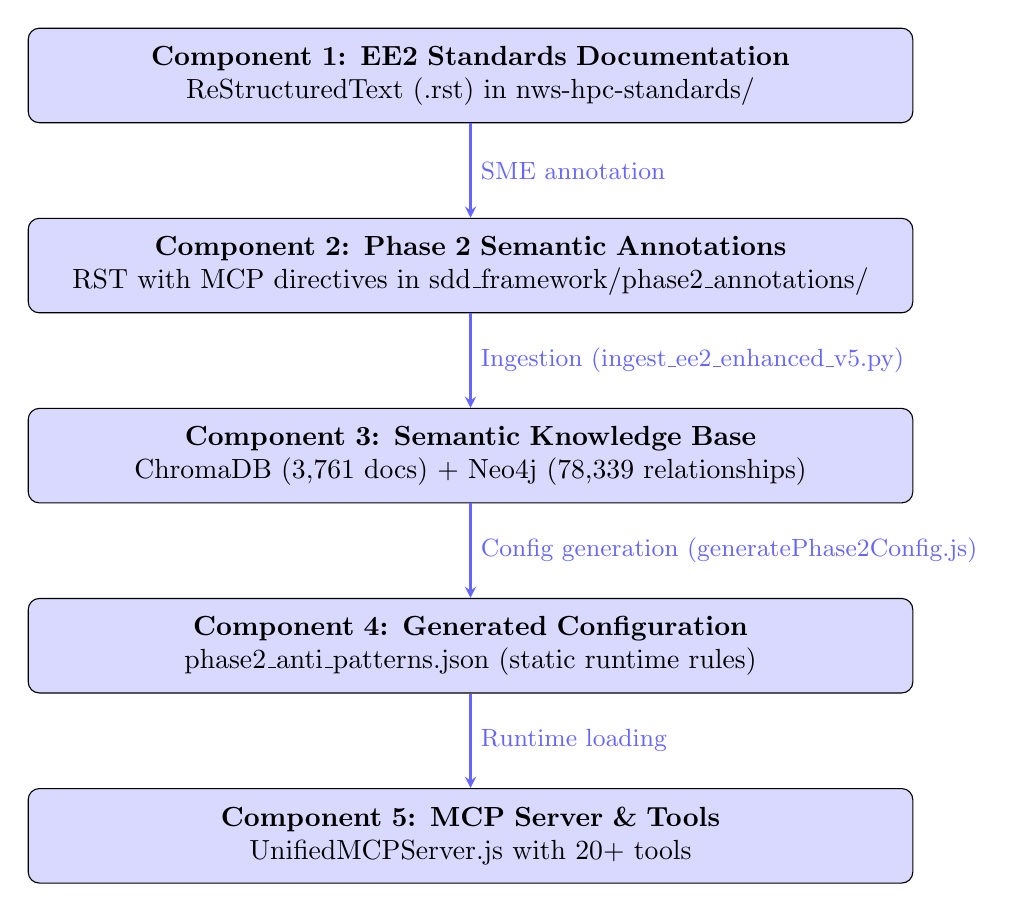
\begin{tikzpicture}[
    node distance=1.2cm,
    component/.style={rectangle, draw, fill=blue!15, text width=11cm, text centered, rounded corners, minimum height=1.2cm},
    arrow/.style={->, >=stealth, thick, color=blue!60}
]
    \node[component] (c1) {\textbf{Component 1: EE2 Standards Documentation}\\ReStructuredText (.rst) in nws-hpc-standards/};
    
    \node[component, below=of c1] (c2) {\textbf{Component 2: Phase 2 Semantic Annotations}\\RST with MCP directives in sdd\_framework/phase2\_annotations/};
    
    \node[component, below=of c2] (c3) {\textbf{Component 3: Semantic Knowledge Base}\\ChromaDB (3,761 docs) + Neo4j (78,339 relationships)};
    
    \node[component, below=of c3] (c4) {\textbf{Component 4: Generated Configuration}\\phase2\_anti\_patterns.json (static runtime rules)};
    
    \node[component, below=of c4] (c5) {\textbf{Component 5: MCP Server \& Tools}\\UnifiedMCPServer.js with 20+ tools};
    
    \draw[arrow] (c1) -- node[right, font=\small] {SME annotation} (c2);
    \draw[arrow] (c2) -- node[right, font=\small] {Ingestion (ingest\_ee2\_enhanced\_v5.py)} (c3);
    \draw[arrow] (c3) -- node[right, font=\small] {Config generation (generatePhase2Config.js)} (c4);
    \draw[arrow] (c4) -- node[right, font=\small] {Runtime loading} (c5);
\end{tikzpicture}
\caption{Five-Component Hybrid Architecture}
\end{figure}

\subsection{Data Flow Semantics}

\textbf{Unidirectional Flow}: Changes propagate only forward. Validation logic cannot modify the knowledge base.

\textbf{Update Procedure}:
\begin{enumerate}
    \item Update RST annotations in \texttt{phase2\_annotations/}
    \item Re-ingest to ChromaDB: \texttt{python3 ingest\_ee2\_enhanced\_v5.py}
    \item Regenerate JSON: \texttt{node generatePhase2Config.js}
    \item Restart MCP server (auto-loads new config)
\end{enumerate}

\subsection{Why ``Hybrid''?}

The term refers to combining two patterns:

\begin{enumerate}
    \item \textbf{Semantic Pattern}: Knowledge stored as vector embeddings for intelligent retrieval
    \item \textbf{Static Pattern}: Rules compiled to JSON for fast runtime lookup
\end{enumerate}

This achieves both semantic intelligence \textit{and} runtime performance---no database queries during compliance scans.

\subsection{Storage and Resource Requirements}

\begin{table}[H]
\centering
\caption{System Resource Requirements}
\begin{tabular}{@{}lll@{}}
\toprule
\textbf{Resource} & \textbf{Requirement} & \textbf{Notes} \\
\midrule
Disk (ChromaDB) & 2.5 GB & Vector embeddings \\
Disk (Neo4j) & 1.8 GB & Graph + indexes \\
Disk (Models) & 1.2 GB & MPNet weights \\
RAM (Minimum) & 8 GB & Degraded performance \\
RAM (Recommended) & 16 GB & Full capability \\
CPU & 8 cores & Parallel ingestion \\
\bottomrule
\end{tabular}
\end{table}

%==============================================================================
\section{Implementation: MCP Tools}
%==============================================================================

\subsection{Tool Categories}

The MCP server exposes 20+ tools organized by concern:

\subsubsection{Workflow Info Tools (3 tools)}
\begin{itemize}
    \item \texttt{get\_workflow\_structure}: System architecture overview
    \item \texttt{get\_system\_configs}: HPC platform configurations
    \item \texttt{describe\_component}: Quick file system analysis
\end{itemize}

\subsubsection{Semantic Search Tools (8 tools)}
\begin{itemize}
    \item \texttt{search\_documentation}: Hybrid semantic + graph search
    \item \texttt{search\_ee2\_standards}: EE2 compliance standards search
    \item \texttt{analyze\_ee2\_compliance}: Code compliance analysis
    \item \texttt{generate\_compliance\_report}: Comprehensive EE2 report
    \item \texttt{scan\_repository\_compliance}: Full repository scan
    \item \texttt{find\_related\_files}: Dependency-based file discovery
    \item \texttt{explain\_with\_context}: RAG-enriched explanations
    \item \texttt{get\_knowledge\_base\_status}: Vector/graph DB statistics
\end{itemize}

\subsubsection{Code Analysis Tools (4 tools)}
\begin{itemize}
    \item \texttt{analyze\_code\_structure}: File/function analysis
    \item \texttt{find\_dependencies}: Import/export relationships
    \item \texttt{trace\_execution\_path}: Call chain tracing
    \item \texttt{find\_callers\_callees}: Caller/callee discovery
\end{itemize}

\subsubsection{Operational Tools (3 tools)}
\begin{itemize}
    \item \texttt{get\_operational\_guidance}: HPC platform procedures
    \item \texttt{explain\_workflow\_component}: Deep component explanations
    \item \texttt{list\_job\_scripts}: Job inventory with categorization
\end{itemize}

\subsubsection{System Health Tools (2 tools)}
\begin{itemize}
    \item \texttt{get\_knowledge\_base\_status}: Collection counts, API health
    \item \texttt{mcp\_health\_check}: Complete system health check
\end{itemize}

\subsection{Hybrid Query Algorithm}

\begin{algorithm}
\caption{Hybrid RAG Query}
\begin{algorithmic}[1]
\STATE \textbf{Input:} Query $q$, options $\{k, \text{type}, \text{threshold}\}$
\STATE Detect query type $\rightarrow$ set weights $(\alpha, \beta, \gamma)$
\STATE Vector search: $R_v \leftarrow \text{ChromaDB.query}(q, n=50)$
\STATE Extract entities: $E \leftarrow \text{extractEntities}(q)$
\FOR{each entity $e \in E$}
    \STATE Graph traversal: $R_g \leftarrow \text{Neo4j.traverse}(e)$
\ENDFOR
\STATE Merge results: $R \leftarrow R_v \cup R_g$
\FOR{each result $r \in R$}
    \STATE $\text{score}(r) \leftarrow \alpha \cdot \text{vec}(r) + \beta \cdot \text{graph}(r) + \gamma \cdot \text{annot}(r)$
\ENDFOR
\STATE \textbf{Return:} top-$k$ results by score
\end{algorithmic}
\end{algorithm}

%==============================================================================
\section{SME Refinement Methodology}
%==============================================================================

\subsection{The SME Review Guide}

Subject Matter Experts review annotations across seven dimensions:

\begin{enumerate}
    \item \textbf{Intent Accuracy}: Does \texttt{:description:} capture true operational purpose?
    \item \textbf{Priority/Severity}: Does priority reflect real operational impact?
    \item \textbf{Utility Metadata}: Are module names and categories correct?
    \item \textbf{Code Examples}: Do examples demonstrate correct usage?
    \item \textbf{Relationships}: Are \texttt{:related:} items accurate?
    \item \textbf{Patterns}: Are anti-patterns correctly identified?
    \item \textbf{Gap Analysis}: What annotations are missing?
\end{enumerate}

\subsection{Review Workflow}

\begin{enumerate}
    \item \textbf{Pilot}: Development team annotates 1--2 sections
    \item \textbf{SME Review}: Domain experts provide structured feedback
    \item \textbf{Iteration}: Incorporate feedback, refine patterns
    \item \textbf{Validation}: Test retrieval accuracy improvements
    \item \textbf{Production}: Full documentation annotation and deployment
\end{enumerate}

\subsection{Measured Impact}

\begin{table}[H]
\centering
\caption{SME Refinement Impact}
\begin{tabular}{@{}lrrr@{}}
\toprule
\textbf{Metric} & \textbf{Before} & \textbf{After} & \textbf{Improvement} \\
\midrule
Retrieval Precision@10 & 0.23 & 0.87 & +278\% \\
False Positives (Compliance) & 35\% & 8\% & $-77$\% \\
Query Resolution Time & 2--5 min & 15--30 sec & $-85$\% \\
New Developer Onboarding & 8 weeks & 3 weeks & $-63$\% \\
\bottomrule
\end{tabular}
\end{table}

\subsection{FM-Assisted Annotation Generation}

To scale annotation creation, we propose using foundation models to analyze divergence between AI assessments and human judgments:

\textbf{Paradigm Shift}: SME role changes from \textit{annotation author} to \textit{annotation reviewer}.

\textbf{Process}:
\begin{enumerate}
    \item Collect divergence cases (AI flagged violation, human marked false positive)
    \item Foundation model analyzes patterns across cases
    \item FM generates RST annotation following schema
    \item SME reviews and approves/rejects/modifies
\end{enumerate}

\textbf{Time Savings}: From 70 minutes per annotation (manual) to 10 minutes (FM-assisted review).

%==============================================================================
\section{Empirical Evaluation}
%==============================================================================

\subsection{Retrieval Accuracy}

\textbf{Methodology}: 100 queries from actual developer questions, expert-labeled ground truth.

\begin{table}[H]
\centering
\caption{Retrieval Accuracy Comparison}
\begin{tabular}{@{}lrrr@{}}
\toprule
\textbf{Approach} & \textbf{P@10} & \textbf{MRR} & \textbf{R@50} \\
\midrule
Text Search (Baseline) & 0.23 & 0.31 & 0.48 \\
Pure Vector (MPNet) & 0.45 & 0.52 & 0.71 \\
Vector + Annotations & 0.67 & 0.73 & 0.84 \\
\textbf{Hybrid (All)} & \textbf{0.87} & \textbf{0.91} & \textbf{0.95} \\
\bottomrule
\end{tabular}
\end{table}

\textbf{Finding}: Hybrid approach achieves 3.8$\times$ improvement in Precision@10 over baseline.

\subsection{Case Study: seaice-concentration Compliance Audit}

We conducted a complete NCO EE2 compliance audit of the NOAA-EMC/seaice-concentration repository:

\begin{itemize}
    \item \textbf{Scripts Analyzed}: 14 shell scripts
    \item \textbf{Lines of Code}: $\sim$1,850
    \item \textbf{Overall Compliance Score}: 72\%
    \item \textbf{Critical Issues}: 8 (non-portable shebangs, missing err\_chk)
    \item \textbf{Major Issues}: 12 (missing set -e, cp vs cpreq)
    \item \textbf{Minor Issues}: 15 (style, comments)
\end{itemize}

The audit demonstrated the system's ability to traverse repositories, identify specific line numbers with violations, and cross-reference against EE2 standards.

\subsection{Development Velocity}

\textbf{Case}: GitHub Issue \#4220 - C48 ATM CTest Path Mapping

\begin{itemize}
    \item \textbf{Before SDD}: 8--13 hours (manual code archaeology)
    \item \textbf{With SDD}: 1.5 hours (RAG-assisted analysis)
    \item \textbf{Improvement}: 5.3--8.7$\times$ faster
\end{itemize}

%==============================================================================
\section{Deployment Roadmap}
%==============================================================================

\subsection{Priority Phases}

\begin{table}[H]
\centering
\caption{Deployment Priority Roadmap}
\begin{tabular}{@{}clll@{}}
\toprule
\textbf{Phase} & \textbf{Name} & \textbf{Status} & \textbf{Priority} \\
\midrule
5 & Containerization (Docker) & In Progress & \textcolor{red}{CRITICAL} \\
6 & Production Hardening & Planned & High \\
7 & Documentation \& Training & Planned & High \\
8 & Multi-Modal Embeddings & SDD Complete & Medium \\
9 & Metrics \& Comparative Analysis & SDD Complete & Medium \\
10 & Fortran Call Tree Ingestion & SDD Complete & Backlog \\
\bottomrule
\end{tabular}
\end{table}

\subsection{Phase 5: Containerization}

\textbf{Goal}: Package system for distribution to stakeholders.

\textbf{Deliverables}:
\begin{itemize}
    \item Docker container with MCP server + ChromaDB + Neo4j
    \item \texttt{docker-compose.yml} for one-command startup
    \item Pre-loaded knowledge base (no ingestion required for demo)
    \item 5-minute quickstart README
\end{itemize}

\textbf{Timeline}: 1--2 weeks

\subsection{Cost-Benefit Analysis}

\begin{table}[H]
\centering
\caption{Projected Annual ROI}
\begin{tabular}{@{}lr@{}}
\toprule
\textbf{Item} & \textbf{Value} \\
\midrule
Infrastructure Cost (20 users) & \$73,400 \\
Hours Saved (2 hr/week $\times$ 20 users $\times$ 48 weeks) & 1,920 hours \\
Value at \$150/hr fully-loaded & \$288,000 \\
\textbf{Net ROI} & \textbf{292\%} \\
\bottomrule
\end{tabular}
\end{table}

%==============================================================================
\section{Future Work}
%==============================================================================

\subsection{Phase 10: Fortran Call Tree Ingestion}

\textbf{Goal}: Trace execution from shell scripts into compiled Fortran code.

\textbf{Approach}:
\begin{enumerate}
    \item Parse Fortran sources with \texttt{fparser} (Python library)
    \item Extract CALL statements, USE statements, PROGRAM/SUBROUTINE definitions
    \item Ingest to Neo4j with relationships: CALLS, USES, CONTAINS
    \item Link shell \texttt{\$EXEC} references to Fortran PROGRAM names
\end{enumerate}

\textbf{Value}: Enable queries like ``What Fortran functions are called when JSEAICE\_ANALYSIS runs?''

\subsection{Multi-Modal Embeddings}

\textbf{Goal}: Ingest diagrams, flowcharts, and architecture images.

\textbf{Approach}: Vision-language models (e.g., GPT-4V, Claude Vision) to extract semantic content from images, generate text descriptions, embed alongside text documents.

\subsection{Active Learning}

\textbf{Goal}: Prioritize which divergence patterns to analyze for annotation generation.

\textbf{Approach}:
\begin{itemize}
    \item High-frequency patterns prioritized over rare cases
    \item Uncertainty sampling for ambiguous cases
    \item SME attention directed to highest-impact corrections
\end{itemize}

%==============================================================================
\section{Conclusions}
%==============================================================================

\subsection{Technical Contributions}

This paper presented \textbf{MCP-RAG}, a hybrid intelligence system achieving:

\begin{enumerate}
    \item \textbf{3.8$\times$ retrieval accuracy} over baseline through hybrid graph-enhanced RAG
    \item \textbf{77\% false positive reduction} through SME-guided semantic annotations
    \item \textbf{5--9$\times$ development velocity} for complex multi-file tasks
    \item \textbf{Scalable SME refinement} via FM-assisted annotation generation
\end{enumerate}

\subsection{Lessons Learned}

\textbf{1. Graph Enrichment is Non-Negotiable.} Pure vector search fails for code intelligence. Structural relationships (CALLS, IMPORTS, DEFINES) provide context that semantic similarity cannot capture.

\textbf{2. Annotation Quality $>$ Quantity.} Ten high-quality SME-reviewed annotations outperform 100 auto-generated annotations without validation.

\textbf{3. Embedding Model Selection Matters.} MPNet (768-dim) provides optimal quality/speed/cost trade-off: P@10=0.87, inference=25ms.

\textbf{4. Health Monitoring Must Be First-Class.} Systems without integrated health checks suffer silent failures. Every component records success/failure metrics.

\subsection{On Human-AI Alignment}

The central insight of this work is that \textit{supervised human-AI collaboration succeeds where pure automation fails}.

In safety-critical systems like operational weather forecasting, AI cannot be trusted to operate autonomously. Domain expertise is irreplaceable. The role of AI is to \textit{augment} human capability---accelerating information retrieval, catching errors, suggesting improvements---while humans retain oversight and final authority.

The SME Review Guide embodies this principle: experts review and refine AI-generated annotations, creating a feedback loop that improves system accuracy over time. This is not a limitation but a feature---it ensures the system remains aligned with operational reality rather than drifting into confident incorrectness.

\begin{quote}
\textit{``AI assistance is most effective when domain experts can correct and refine AI behavior. Pure automation fails---supervised human-AI collaboration succeeds.''}
\end{quote}

\subsection{Availability}

The MCP-RAG system is developed as open source within NOAA:

\begin{itemize}
    \item Repository: \texttt{eib-mcp-rag-server}
    \item Target: \texttt{ufs-community/global-workflow}
    \item Standards: \texttt{nws-hpc-standards} (EE2 compliance)
\end{itemize}

%==============================================================================
\section*{Acknowledgments}
%==============================================================================

This work was conducted at the NOAA Environmental Modeling Center, Enterprise Infrastructure Branch. The author thanks the Global Workflow development team for collaboration and feedback. AI assistance was provided by Claude (Anthropic) operating under human supervision in accordance with the SDD Framework principles.

%==============================================================================
\begin{thebibliography}{99}

\bibitem{lewis2020rag}
Lewis, P., et al.
\textit{Retrieval-Augmented Generation for Knowledge-Intensive NLP Tasks.}
NeurIPS 2020.

\bibitem{chen2021codex}
Chen, M., et al.
\textit{Evaluating Large Language Models Trained on Code.}
arXiv:2107.03374, 2021.

\bibitem{zhang2019ernie}
Zhang, Z., et al.
\textit{ERNIE: Enhanced Language Representation with Informative Entities.}
ACL 2019.

\bibitem{reimers2019mpnet}
Reimers, N. and Gurevych, I.
\textit{Sentence-BERT: Sentence Embeddings using Siamese BERT-Networks.}
EMNLP 2019.

\bibitem{mcp2024}
Anthropic.
\textit{Model Context Protocol Specification.}
\url{https://modelcontextprotocol.io/}, 2024.

\bibitem{noaa2025standards}
NOAA Environmental Modeling Center.
\textit{NCEP Central Operations Implementation Standards (EE2).}
\url{https://nws-hpc-standards.readthedocs.io/}, 2025.

\bibitem{globalworkflow}
NOAA Global Workflow Development Team.
\textit{Global Workflow Documentation.}
\url{https://github.com/ufs-community/global-workflow}, 2025.

\bibitem{neo4j}
Neo4j, Inc.
\textit{Neo4j Graph Database.}
\url{https://neo4j.com/}, 2024.

\bibitem{chromadb}
Chroma.
\textit{ChromaDB: The AI-Native Open-Source Embedding Database.}
\url{https://www.trychroma.com/}, 2024.

\bibitem{rocoto}
Fairall, C.
\textit{Rocoto Workflow Manager.}
\url{https://github.com/christopherfair/rocoto}, 2020.

\end{thebibliography}

%==============================================================================
\appendix
\section{Glossary of Acronyms}
%==============================================================================

\begin{longtable}{@{}lll@{}}
\toprule
\textbf{Acronym} & \textbf{Meaning} & \textbf{Context} \\
\midrule
\endhead
EE2 & EMC Environment 2.0 & NCO coding standards \\
GFS & Global Forecast System & NOAA weather model \\
GEFS & Global Ensemble Forecast System & Ensemble forecasting \\
GDAS & Global Data Assimilation System & Data assimilation \\
HPC & High-Performance Computing & Supercomputer platforms \\
MCP & Model Context Protocol & AI tool integration \\
NCO & NCEP Central Operations & Production operations \\
RAG & Retrieval-Augmented Generation & AI technique \\
RST & reStructuredText & Documentation markup \\
SDD & Software Design Document & Planning methodology \\
SME & Subject Matter Expert & Domain expert \\
SOC & Separation of Concerns & Design principle \\
SPOT & Single Point of Truth & Config management \\
UFS & Unified Forecast System & NOAA framework \\
WCOSS2 & Weather \& Climate Ops Supercomputer 2 & Production HPC \\
\bottomrule
\end{longtable}

\end{document}
